\documentclass{article}
\usepackage{mathtools}
\usepackage[margin=0.95in]{geometry}
%\renewcommand{\familydefault}{\sfdefault}
\usepackage{amssymb}
\usepackage{cancel}
\usepackage{tikz-cd}
\usepackage{tikz}
\usepackage{caption}
\usepackage{pgfplots}
\usepackage{pgf}
\usepackage{centernot}
\usetikzlibrary{arrows,automata}
\usepackage{booktabs}
\usepackage{enumerate}
\usepackage{multirow}
%\usepackage{bbold}
\usepackage{changepage}
\pgfplotsset{compat = newest}
\usepackage{gensymb}
\usepackage{array}
\usepackage{makecell}
\usepackage[utf8]{inputenc}
\usepackage[english]{babel}
\usepackage{stmaryrd}
\usepackage[table]{xcolor}
\usepackage{listings}
\definecolor{background}{RGB}{255,248,197}
\definecolor{gb}{RGB}{66, 133, 244}
\definecolor{gr}{RGB}{234, 67, 53}
\definecolor{gy}{RGB}{251, 188, 5}
\definecolor{gg}{RGB}{52, 168, 83}
\usepackage{color}
\usepackage{hyperref}
\hypersetup{colorlinks=true, linkcolor=black,
urlcolor=blue, linktoc=all}
\setcounter{MaxMatrixCols}{20}
\usepackage{witharrows}
\usepackage{graphicx}
\usepackage{bm}
\usepackage{tabu}
\usepackage[most]{tcolorbox} %[enhanced,boxrule=0pt, frame hidden, sharp corners, borderline west={3pt}{-1.5pt}{black},breakable]
\usepackage{amsthm}
\usepackage{xfrac}
\usepackage{commath}
\usepackage{dirtytalk}
\usepackage{ytableau}
\newcommand{\inv}{^{-1}}
\newcommand{\qtq}[1]{\quad\text{#1}\quad}
\newcommand{\txt}[1]{\ \text{#1}\ }
\renewcommand{\ker}{\text{ker}}
\newcommand{\coker}{\text{coker}}
\newcommand{\Cor}{\text{Cor}_G(H)}
\newcommand{\ind}{\xrightarrow{d}}
\newcommand{\inp}{\xrightarrow{P}}
\newcommand{\almo}{\xrightarrow{\text{a.s}}}
\newcommand{\vecv}{\vec{v}}
\newcommand{\vecu}{\vec{u}}
\newcommand{\vecw}{\vec{w}}
\newcommand{\zmod}[1]{\Z/ #1 \Z}
\newcommand{\floor}[1]{\lfloor #1 \rfloor}
\newcommand{\lip}{\langle}
\newcommand{\rip}{\rangle}
\DeclareSymbolFont{symbolsC}{U}{txsyc}{m}{n}
\DeclareMathSymbol{\indep}{\mathrel}{symbolsC}{121}
\newcommand{\newpar}{\vspace{8pt}}
\renewcommand{\phi}{\varphi}
\newcommand{\ptwo}{p_\Lambda^{(2)}}
\newcommand{\pthree}{p_\Lambda^{(3)}}
\renewcommand{\epsilon}{\varepsilon}
\renewcommand{\theta}{\vartheta}
\DeclareMathOperator*{\argmax}{arg\,max}
\DeclareMathOperator{\deg}{deg}
\DeclareMathOperator*{\argmin}{arg\,min}
\DeclareMathOperator*{\limeaunf}{limea\"unf}
\newcommand{\Ree}{\text{Re}}
\newcommand{\Imm}{\text{Im}}
\newcommand{\iid}{\stackrel{\text{i.i.d}}{\sim}}
\newcommand{\rank}{\text{rank}}
\newcommand{\Span}{\text{span}}
\newcommand{\Int}{\text{Int}}
\newcommand{\Clos}{\text{Clos}}
\newcommand{\ideal}{\mathfrak{A}}
\newcommand{\idm}{\mathfrak{m}}
\newcommand{\idn}{\mathfrak{n}}
\newcommand{\idp}{\mathfrak{p}}
\newcommand{\idq}{\mathfrak{q}}
\newcommand{\limty}{\lim_{n\to\infty}}
\newcommand{\seq}[1]{(#1_n)_{n\geq1}}
\newcommand{\leteps}{\text{Let } \varepsilon > 0}
\renewcommand{\char}{\text{char}}
\newcommand{\mb}[1]{\bm{#1}}
\newcommand{\nil}{\text{nil}}
\newcommand{\code}[1]{\texttt{#1}}
\newcommand\bigzero{\makebox(0,0){\text{\huge0}}}
\renewcommand{\div}{\text{div}}
\newcommand{\R}{\mathbb{R}}
\newcommand{\N}{\mathbb{N}}
\newcommand{\C}{\mathbb{C}}
\renewcommand{\P}{\mathbb{P}}
\newcommand{\F}{\mathcal{F}}
\newcommand{\Z}{\mathbb{Z}}
\newcommand{\Q}{\mathbb{Q}}
\newcommand{\I}{\mathbb{I}}
\newcommand{\T}{\mathbb{T}}
\newcommand{\E}{\mathbb{E}}
\renewcommand{\S}{\mathbb{S}}
\newcommand{\zd}{\text{zd}}
\newcommand{\normal}{\vartriangleleft}
\newcommand{\Aut}{\text{Aut}}
\newcommand{\Inn}{\text{Inn}}
\newcommand{\ds}{\displaystyle}
\newcommand{\Vol}{\text{Vol}}
\newcommand{\sip}{(\ \ \mid\ \ )}
\newcommand{\intfin}{\int_{-\infty}^{\infty}}
\newcommand{\sumi}[1]{\sum_{i=1}^{#1}}
\newcommand{\ren}[1]{\mathbb{R}^{#1}}
\newcommand{\con}[1]{\mathbb{C}^{#1}}
\newcommand{\chisq}[1]{\chi^2_{#1}}
\newcommand{\orthcomp}{^{\perp}}
\newcommand{\im}{\text{im}}
\newenvironment{graytext}{\color{gray}}{\ignorespacesafterend}
\newcommand{\cov}{\text{cov}}
\newcommand{\var}{\text{var}}
\renewcommand{\l}{\left}
\renewcommand{\r}{\right}
\definecolor{codegreen}{rgb}{0,0.6,0}
\definecolor{codegray}{rgb}{0.5,0.5,0.5}
\definecolor{codepurple}{rgb}{0.58,0,0.82}
\definecolor{backcolour}{rgb}{0.95,0.95,0.92}
\mathtoolsset{showonlyrefs} 
\usepackage[utf8]{inputenc}
\setlength\parindent{0pt}

\lstdefinestyle{mystyle}{
    backgroundcolor=\color{backcolour},   
    commentstyle=\color{codegreen},
    keywordstyle=\color{magenta},
    numberstyle=\tiny\color{codegray},
    stringstyle=\color{codepurple},
    basicstyle=\ttfamily\footnotesize,
    breakatwhitespace=false,         
    breaklines=true,                 
    captionpos=b,                    
    keepspaces=true,                 
    numbers=left,                    
    numbersep=5pt,                  
    showspaces=false,                
    showstringspaces=false,
    showtabs=false,                  
    tabsize=2
}

\lstdefinestyle{python2}{
    language=Python,
    basicstyle=\ttfamily\small,
    keywordstyle=\color{blue},
    commentstyle=\color{gray},
    stringstyle=\color{red!60!black},
    showstringspaces=false,
    frame=single,
    numbers=left,
    numberstyle=\tiny\color{gray},
    tabsize=4,
    breaklines=true,
}
\usepackage{float}

\title{\textbf{\textsf{Stat 175: Homework 4}}}
\author{\textsf{Matt Krasnow}}
\date{\textsf{Spring 2026}}

\begin{document}

\maketitle

Please submit your solutions to \href{https://www.gradescope.com/courses/1244242}{\underline{Gradescope}} by \textbf{Friday, March $\bm{6}^{\text{th}}$, 11:59 pm}.\newpar

\begin{tcolorbox}[colback = gray!16, enhanced, boxrule=0pt, frame hidden, sharp corners, borderline west={3pt}{-1.5pt}{black!80},breakable]
\textbf{Exercise 1 (Modularity and Cliques).} Consider a graph $G$ with four cliques of size 4, and exactly one edge between each
neighboring clique:
\begin{center}
    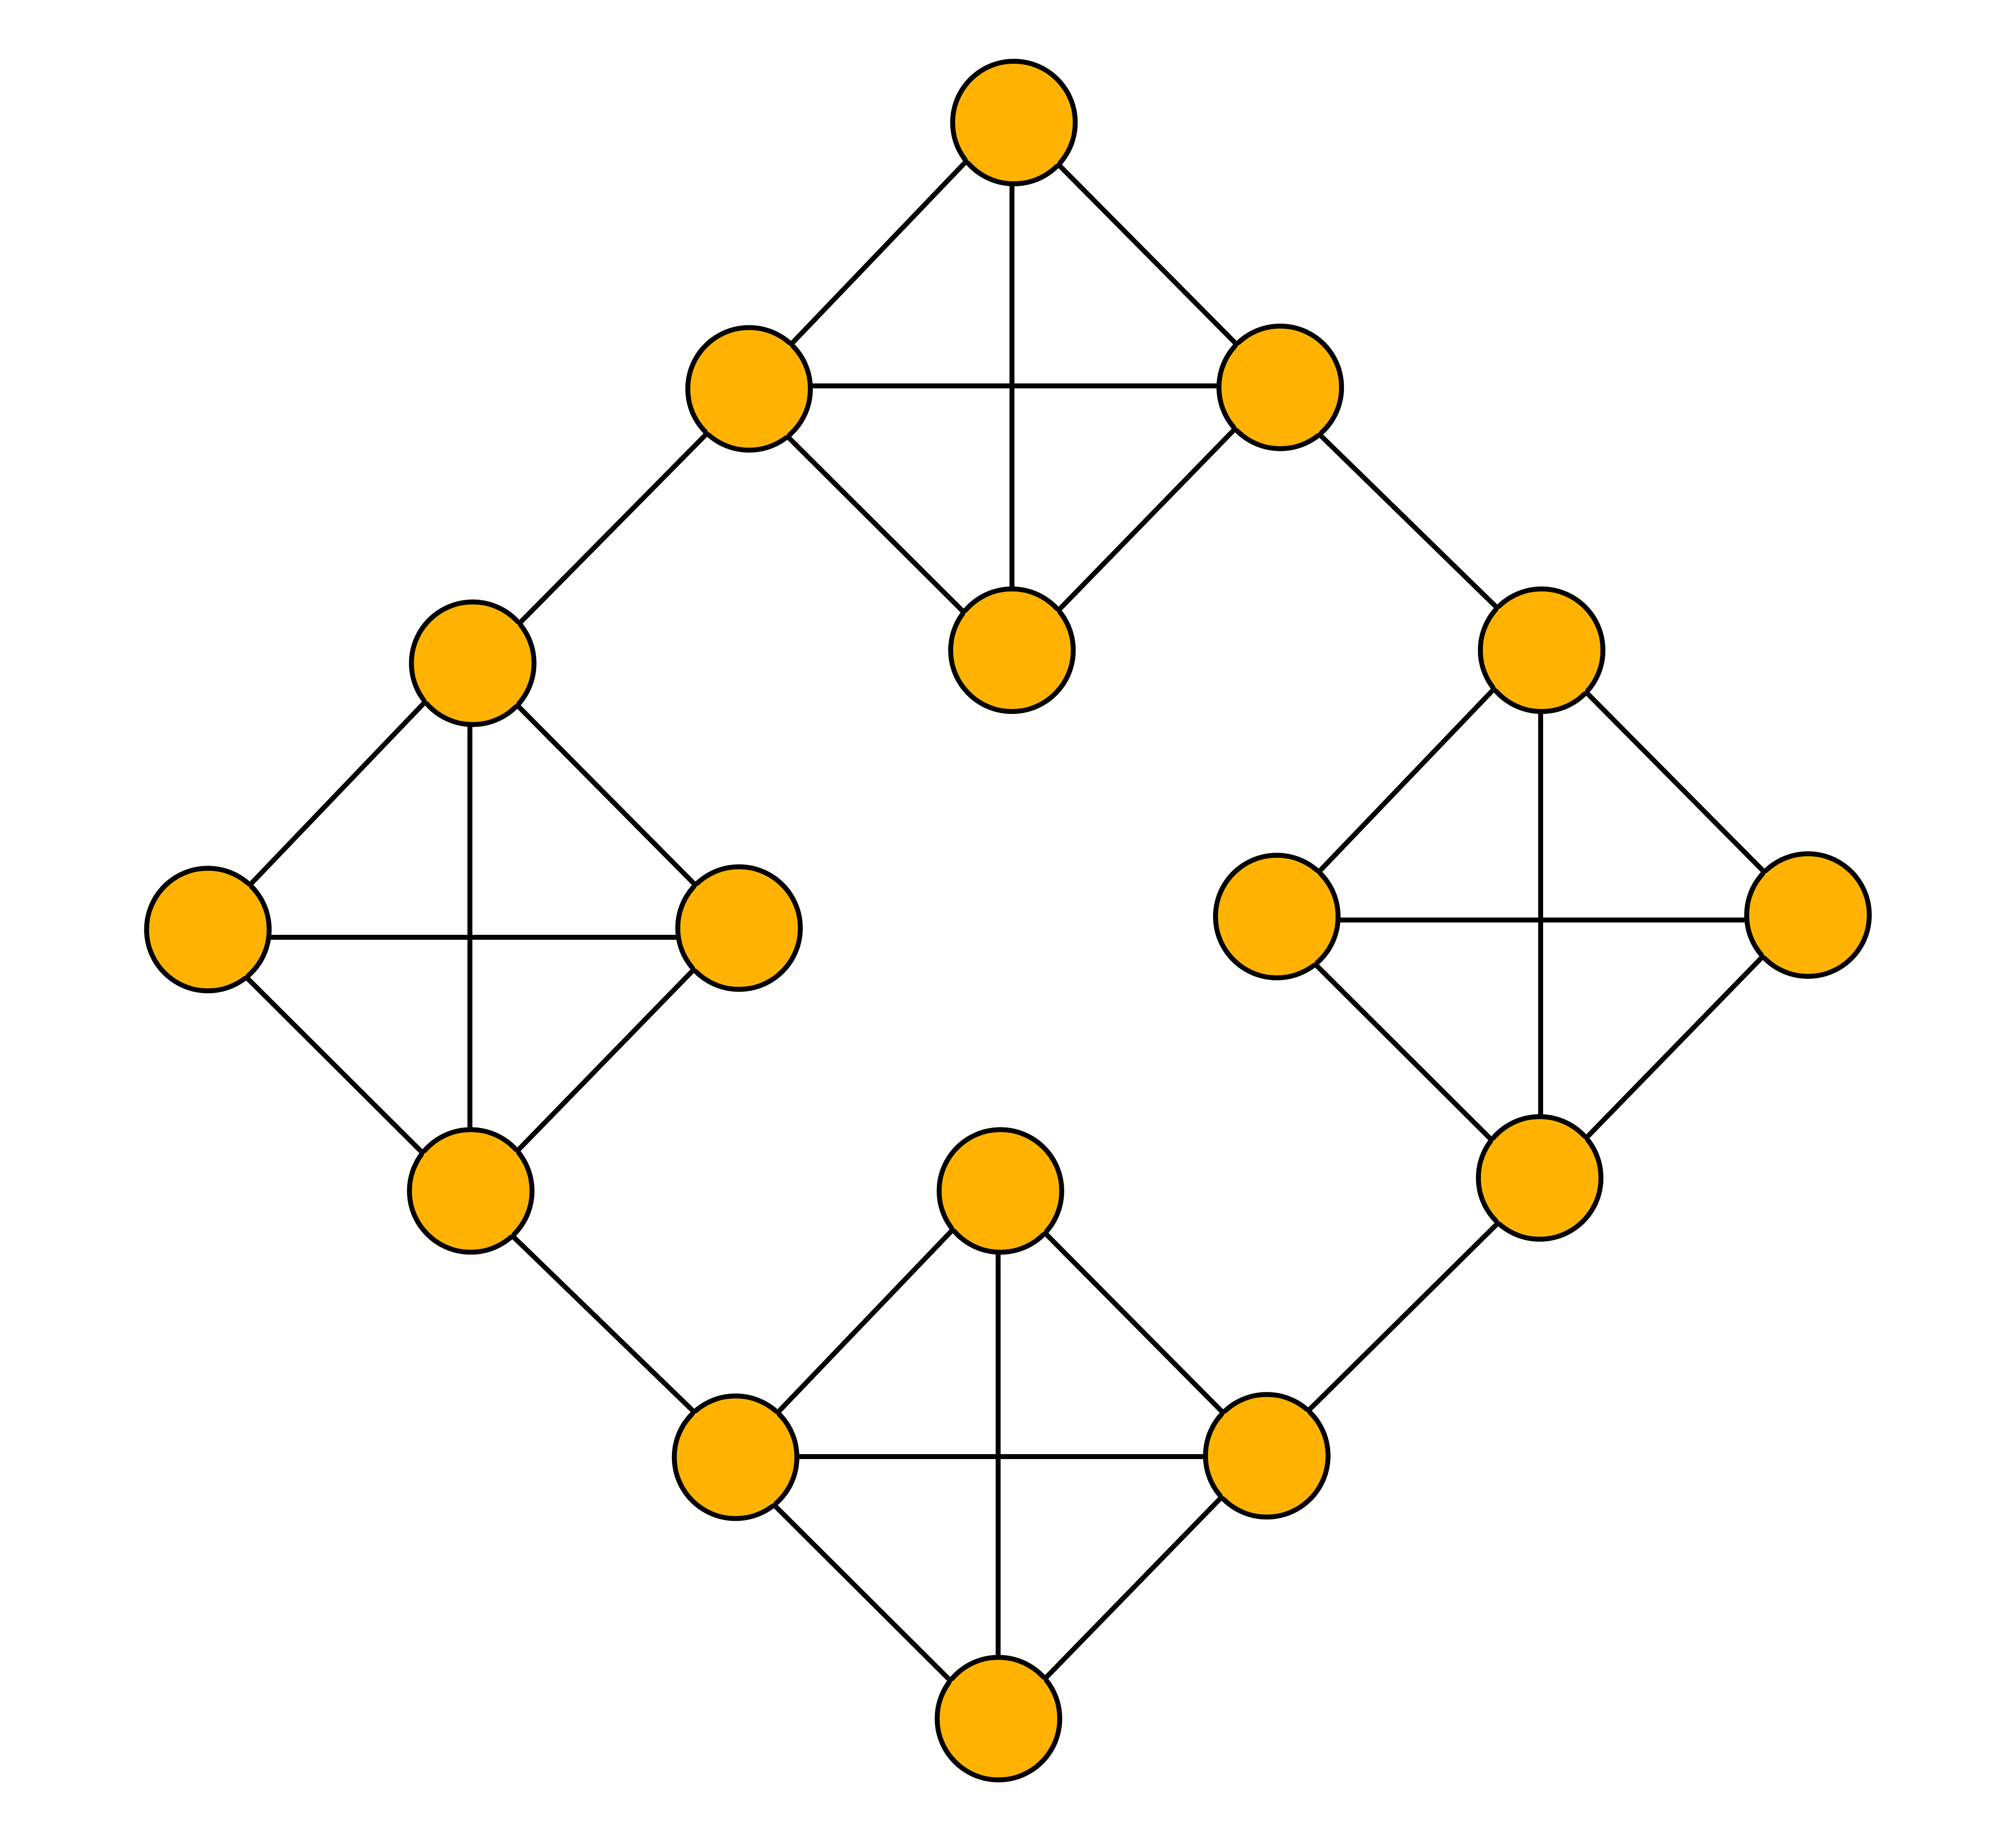
\includegraphics[width=0.35\textwidth]{Figures/clique.png}
\end{center}

Let's do Louvain community detection on this graph. Suppose that all the vertices in each separate clique have been assigned to the same community, meaning we consider four communities total.
\begin{enumerate}[$(a)$]
    \item  Prove that when each vertex in the same clique is assigned to the same community, then no gain in modularity can be made by moving a vertex.
    \item Draw the aggregated network.
    \item Consider the Louvain algorithm applied to the aggregated network. At each level
of the algorithm, the communities of the previous level are treated as nodes of
the new network. Given the initial community assignments, would you want to
move any of the nodes at any level of the algorithm? Explain your reasoning.
\end{enumerate}
\end{tcolorbox}

\begin{tcolorbox}[colback=white, colframe=black!70, title=\textbf{Solution to Exercise 1}, breakable]

\textbf{Setup.} The graph $G$ consists of four cliques $C_1,C_2,C_3,C_4$, each isomorphic to $K_4$, arranged in a ring with one bridge edge between each consecutive pair. Thus:
\begin{itemize}
\item Each clique has $\binom{4}{2}=6$ internal edges.
\item There are $4$ bridge edges (one per adjacent clique pair in the ring).
\item Total edges: $m = 4\cdot 6 + 4 = 28$, so $2m = 56$.
\item Each clique has exactly $2$ bridge vertices (one bridge to each neighboring clique) and $2$ non-bridge vertices.
\item A bridge vertex has degree $k = 3 + 1 = 4$ (3 within its clique, 1 bridge).
\item A non-bridge vertex has degree $k = 3$ (all within its clique).
\item The sum of degrees within each clique is $\Sigma_C = 2\cdot 4 + 2\cdot 3 = 14$.
\end{itemize}

\begin{enumerate}[(a)]
\item \textbf{Prove that no single-vertex move improves modularity.}

Recall that the change in modularity when moving vertex $v$ from its current community $C$ to a different community $C'$ is
\[
\Delta Q = \frac{1}{m}\l[k_{v\to C'} - \frac{\Sigma_{C'}\cdot k_v}{2m}\r] - \frac{1}{m}\l[k_{v\to C\setminus v} - \frac{(\Sigma_C - k_v)\cdot k_v}{2m}\r],
\]
where $k_{v\to X}$ denotes the number of edges from $v$ to vertices in community $X$, $k_v$ is the degree of $v$, and $\Sigma_X = \sum_{i\in X} k_i$ is the sum of degrees in community $X$.

We consider all possible vertex types and target communities.

\medskip
\textbf{Case 1: $v$ is a non-bridge vertex (degree $k_v = 3$).}

All three of $v$'s neighbors lie in its own clique $C$. For \emph{any} other community $C'$:
\[
k_{v\to C'} = 0, \qquad k_{v\to C\setminus v} = 3, \qquad \Sigma_{C'} = 14, \qquad \Sigma_C - k_v = 14-3 = 11.
\]
Thus
\[
\Delta Q = \frac{1}{28}\l[0 - \frac{14\cdot 3}{56}\r] - \frac{1}{28}\l[3 - \frac{11\cdot 3}{56}\r]
= \frac{1}{28}\l[-\frac{3}{4}\r] - \frac{1}{28}\l[3 - \frac{33}{56}\r]
= \frac{1}{28}\l[-\frac{3}{4} - 3 + \frac{33}{56}\r].
\]
Computing the bracket:
\[
-\frac{3}{4} - 3 + \frac{33}{56} = -\frac{42}{56} - \frac{168}{56} + \frac{33}{56} = -\frac{177}{56}.
\]
So $\Delta Q = -\dfrac{177}{56\cdot 28} = -\dfrac{177}{1568} < 0$.

\medskip
\textbf{Case 2: $v$ is a bridge vertex (degree $k_v = 4$) moved to the neighboring clique $C'$ it bridges to.}

Here $v$ has 3 neighbors in $C$ and 1 neighbor in $C'$:
\[
k_{v\to C'} = 1, \qquad k_{v\to C\setminus v} = 3, \qquad \Sigma_{C'} = 14, \qquad \Sigma_C - k_v = 14-4 = 10.
\]
Thus
\[
\Delta Q = \frac{1}{28}\l[1 - \frac{14\cdot 4}{56}\r] - \frac{1}{28}\l[3 - \frac{10\cdot 4}{56}\r]
= \frac{1}{28}\l[1 - 1\r] - \frac{1}{28}\l[3 - \frac{5}{7}\r]
= 0 - \frac{1}{28}\cdot \frac{16}{7}
= -\frac{16}{196} = -\frac{4}{49} < 0.
\]

\medskip
\textbf{Case 3: $v$ is a bridge vertex (degree $k_v = 4$) moved to a non-neighboring community $C''$.}

Here $v$ has no neighbors in $C''$:
\[
k_{v\to C''} = 0, \qquad k_{v\to C\setminus v} = 3, \qquad \Sigma_{C''} = 14, \qquad \Sigma_C - k_v = 10.
\]
Thus
\[
\Delta Q = \frac{1}{28}\l[0 - \frac{14\cdot 4}{56}\r] - \frac{1}{28}\l[3 - \frac{10\cdot 4}{56}\r]
= \frac{1}{28}\l[-1\r] - \frac{1}{28}\l[\frac{16}{7}\r]
= -\frac{1}{28} - \frac{16}{196} = -\frac{1}{28} - \frac{4}{49} < 0.
\]

\medskip
In every case, $\Delta Q < 0$. Therefore, \boxed{\text{no single-vertex move can increase the modularity.}} \qed

\item \textbf{Draw the aggregated network.}

In the Louvain algorithm, after the first phase each community is collapsed into a single super-node. Internal edges become self-loops (with weight equal to the number of internal edges), and bridge edges between communities become weighted edges between super-nodes.

Each clique $C_i$ becomes a node with a self-loop of weight $6$ (from $\binom{4}{2}=6$ internal edges). The four bridge edges become edges of weight $1$ connecting neighboring super-nodes in a cycle.

\begin{center}
\begin{tikzpicture}[scale=1.8, every node/.style={draw, circle, minimum size=22pt, inner sep=1pt, font=\small}]
  \node (T) at (0,1.3) {$C_1$};
  \node (L) at (-1.3,0) {$C_2$};
  \node (R) at (1.3,0) {$C_4$};
  \node (B) at (0,-1.3) {$C_3$};

  % Bridge edges (cycle)
  \draw[thick] (T) -- node[draw=none, fill=white, minimum size=0pt, inner sep=1pt, font=\scriptsize, pos=0.5] {$1$} (L);
  \draw[thick] (L) -- node[draw=none, fill=white, minimum size=0pt, inner sep=1pt, font=\scriptsize, pos=0.5] {$1$} (B);
  \draw[thick] (B) -- node[draw=none, fill=white, minimum size=0pt, inner sep=1pt, font=\scriptsize, pos=0.5] {$1$} (R);
  \draw[thick] (R) -- node[draw=none, fill=white, minimum size=0pt, inner sep=1pt, font=\scriptsize, pos=0.5] {$1$} (T);

  % Self-loops
  \draw[thick] (T) to[out=60,in=120,looseness=8] node[draw=none, fill=white, minimum size=0pt, inner sep=1pt, font=\scriptsize, above=2pt] {$6$} (T);
  \draw[thick] (L) to[out=150,in=210,looseness=8] node[draw=none, fill=white, minimum size=0pt, inner sep=1pt, font=\scriptsize, left=2pt] {$6$} (L);
  \draw[thick] (R) to[out=-30,in=30,looseness=8] node[draw=none, fill=white, minimum size=0pt, inner sep=1pt, font=\scriptsize, right=2pt] {$6$} (R);
  \draw[thick] (B) to[out=-120,in=-60,looseness=8] node[draw=none, fill=white, minimum size=0pt, inner sep=1pt, font=\scriptsize, below=2pt] {$6$} (B);
\end{tikzpicture}
\end{center}

The aggregated network is a weighted cycle $C_4$ on four super-nodes, where each node has a self-loop of weight $6$ and each edge in the cycle has weight $1$.

\item \textbf{Would Louvain merge any communities at subsequent levels?}

At the second level, Louvain operates on the aggregated network above. Each super-node $i$ starts as its own community. We check whether merging two adjacent super-nodes improves modularity.

In the weighted aggregated network, the \emph{strength} (weighted degree) of each node is
\[
s_i = 2\cdot 6 + 1 + 1 = 14,
\]
where the self-loop of weight $6$ contributes $2\times 6 = 12$ to the strength, and the two cycle edges each contribute $1$. The total weight is $m' = \frac{1}{2}\sum_i s_i = \frac{4\cdot 14}{2}= 28$, so $2m' = 56$.

Consider merging two adjacent super-nodes $i$ and $j$ (connected by an edge of weight $1$). Moving node $i$ into node $j$'s community:
\[
\Delta Q = \frac{1}{m'}\l[k_{i\to j} - \frac{s_j\cdot s_i}{2m'}\r] = \frac{1}{28}\l[1 - \frac{14\cdot 14}{56}\r] = \frac{1}{28}\l[1 - 3.5\r] = \frac{-2.5}{28} < 0.
\]

For non-adjacent super-nodes (e.g., $C_1$ and $C_3$), the edge weight between them is $0$:
\[
\Delta Q = \frac{1}{28}\l[0 - \frac{14\cdot 14}{56}\r] = \frac{-3.5}{28} < 0.
\]

Since every possible merge decreases modularity, \textbf{no moves are made} at the second level. The algorithm terminates, and the partition into the original four cliques is the final output.

\medskip
\textbf{Remark (Resolution Limit).} This example illustrates the \emph{resolution limit} of modularity. The four-clique ring is a local optimum of modularity under the Louvain algorithm: no single-vertex move (level 1) and no community merge (level 2+) improves the objective. However, one could argue that merging pairs of adjacent cliques into two larger communities might yield a partition that is globally competitive. Louvain's greedy, local nature prevents it from discovering such rearrangements, demonstrating that it can get stuck at suboptimal local maxima.

\end{enumerate}
\end{tcolorbox}

\vspace{12pt}

\begin{tcolorbox}[colback = gray!16, enhanced, boxrule=0pt, frame hidden, sharp corners, borderline west={3pt}{-1.5pt}{black!80},breakable]
\textbf{Exercise 2 (Protein Data Community Detection).} In this exercise, you will explore the community structure of the Yeast protein-protein interaction network using the Louvain algorithm and spectral graph embedding. 
\begin{enumerate}[$(a)$]
    \item Download the $\code{yeast.graphml}$ file from the ``HW 4'' folder and place it in your code file's working directory. Then run the following two commands in Python to load our dataset:
    \begin{align}
        &\hspace{-200pt}\code{import igraph as ig}\\
        &\hspace{-200pt}\code{G = ig.Graph.Read\_GraphML("yeast.graphml")}
    \end{align}
    For the rest of this problem, we will be working with $\code{igraph}$ to manipulate graphs on top of our standard $\code{networkx}$. For a manual on how to do some basic commands in this library, \href{https://igraph.org/python/tutorial/0.9.9/tutorial.html}{\underline{click the link here}}. Otherwise, feel free to use AI to learn new $\code{igraph}$ commands. Some important ones you should use to explore the data for yourself are $\code{G.vcount()}$ and $\code{G.ecount()}$ (number of nodes/edges), and $\code{G.attributes()}$, $\code{G.vs.attributes()}$, and $\code{G.es.attributes()}$ (attributes of the graph, nodes, and edges, respectively).
    \item Run the Louvain algorithm on the network and report both the modularity of the detected communities and the overall number of communities.

    (\textit{Hint: Louvain is run via} $\code{G.community\_multilevel()}$, \textit{and you can use} $\code{dir()}$ \textit{on the output to see all accessible attribute names such as modularity})
    \item Visualize the aggregated network. You might need to import $\code{cairocffi}$ to do this in $\code{igraph}$, or you can transfer the graph to $\code{networkx}$ and use our old visualization methods.
\item We want to consider another approach to community detection by embedding the nodes of the network into a low-dimensional space. To do so, we use the Laplacian Spectral Clustering method seen in lecture. Do this to obtain three different embeddings of dimensions $d = 3, 10,$ and $40$.

(\textit{Hint: In Section 2, we did exactly this for only a single dimension by getting the Fiedler vector $e_2$. You can use this same method, just now with dimensions 3, 10, and 40.})

\item Now that you have your three different embeddings, run $k$-means clustering on them all to detect communities. Your value of $k$ should be the number of communities you reported in part $(b)$.

\item Compare the community structure obtained from the Louvain algorithm with that obtained from the spectral embedding. Discuss the similarities and differences between the two.
\end{enumerate}
\end{tcolorbox}

\begin{tcolorbox}[colback=white, colframe=black!70, title=\textbf{Solution to Exercise 2}, breakable]

\begin{enumerate}[(a)]

\item We load the yeast protein-protein interaction network and restrict to the largest connected component. The resulting graph has $\mathbf{1458}$ \textbf{nodes} and $\mathbf{1948}$ \textbf{edges}. The graph has vertex attribute \code{id}; it is undirected and simple.

\begin{lstlisting}[style=python2]
import igraph as ig
G = ig.Graph.Read_GraphML("yeast.graphml")
G = G.connected_components().giant()
G = G.simplify()
print(G.vcount(), G.ecount())  # 1458 nodes, 1948 edges
print(G.vs.attributes())       # ['id']
print(G.es.attributes())       # []
\end{lstlisting}

\item We run the Louvain algorithm via \code{G.community\_multilevel()}:
\begin{lstlisting}[style=python2]
louvain = G.community_multilevel()
print(louvain.modularity)  # 0.8168
print(len(louvain))         # 29 communities
\end{lstlisting}
\begin{itemize}
    \item \textbf{Modularity}: $Q = 0.8168$.
    \item \textbf{Number of communities}: $k = 29$.
\end{itemize}
The high modularity indicates strong community structure. Community sizes range from 17 to 123 vertices.

\item The aggregated network collapses each of the 29 Louvain communities into a single super-node. Edge weights between super-nodes equal the number of inter-community edges in the original graph. Figure~\ref{fig:ex2c} shows this aggregated network (node sizes proportional to community size).

\begin{lstlisting}[style=python2]
agg = louvain.cluster_graph(combine_edges=dict(weight="sum"))
\end{lstlisting}

\begin{figure}[H]
  \centering
  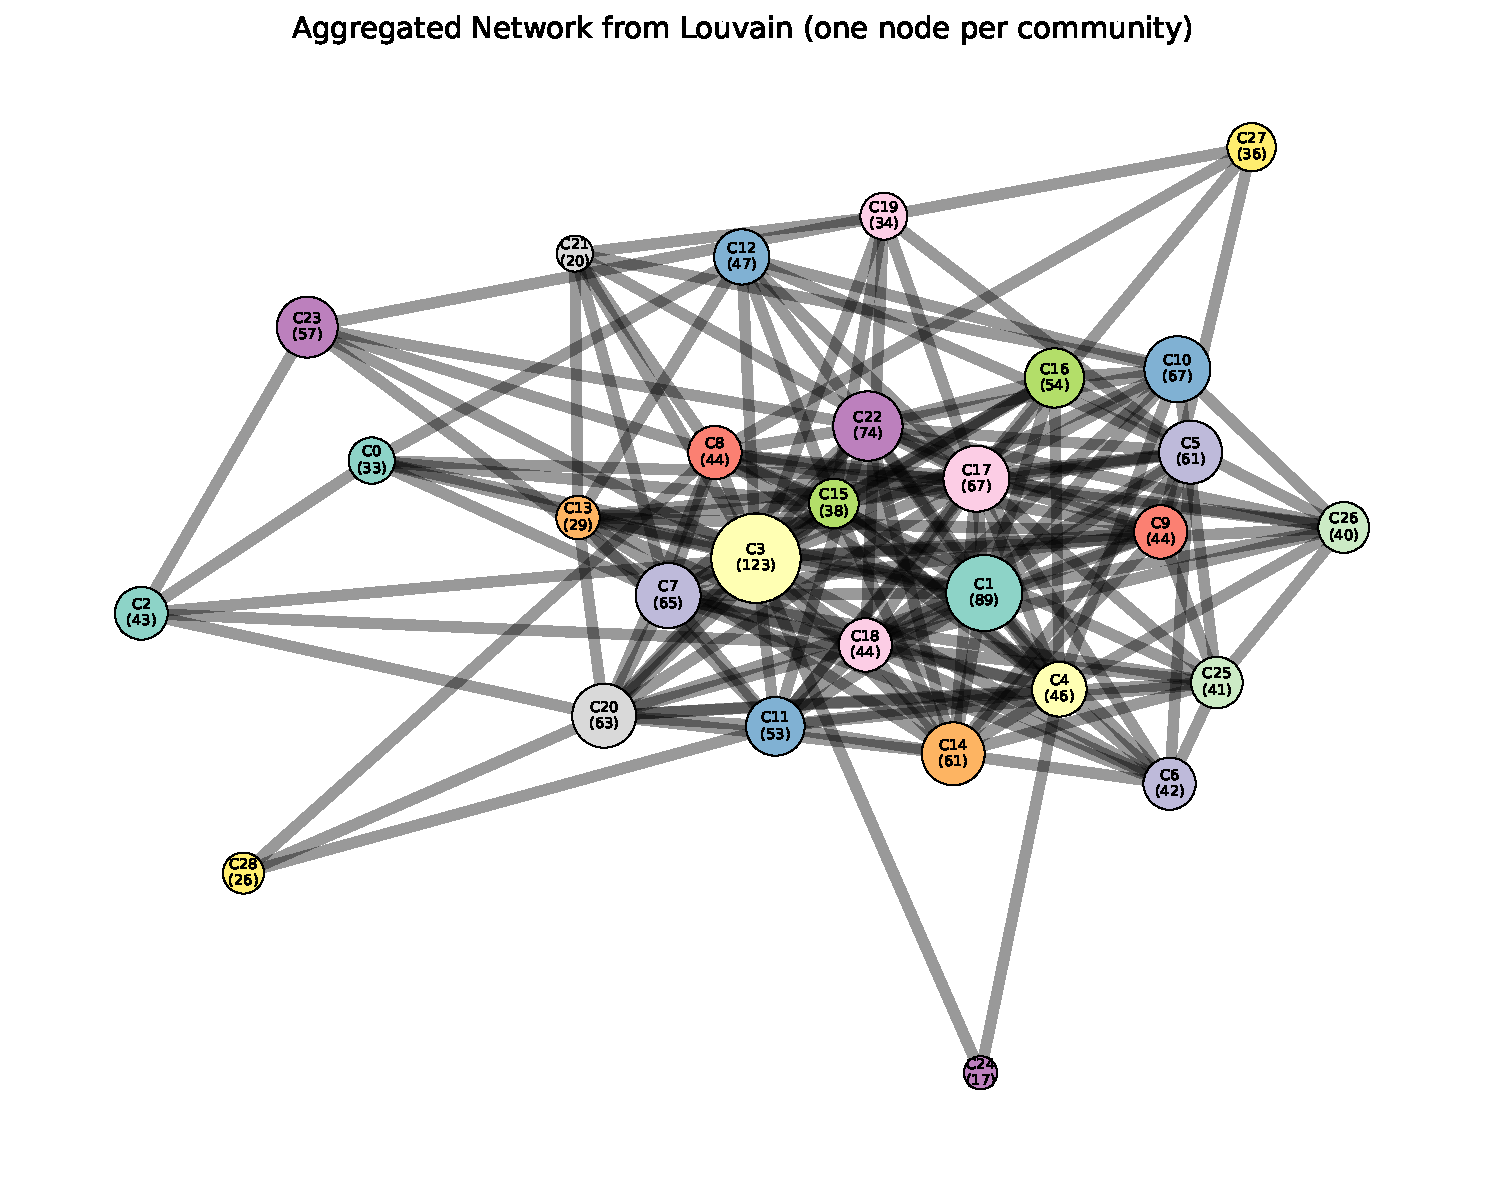
\includegraphics[width=0.75\textwidth]{Figures/ex2c_aggregated.pdf}
  \caption{Aggregated network from Louvain: each node represents one of the 29 communities.}
  \label{fig:ex2c}
\end{figure}

\item We compute the unnormalized graph Laplacian $L = D - A$ and find its eigenvectors. For embedding dimension $d$, we use eigenvectors $e_2, e_3, \ldots, e_{d+1}$ (corresponding to the $d$ smallest non-zero eigenvalues of $L$). Each vertex $i$ is embedded as $(e_{2,i}, e_{3,i}, \ldots, e_{d+1,i}) \in \R^d$.

\begin{lstlisting}[style=python2]
from scipy.sparse.linalg import eigsh
L = D - A   # graph Laplacian
eigenvalues, eigenvectors = eigsh(L, k=41, which='SM')
# For d=3:  X_3  = eigenvectors[:, 1:4]
# For d=10: X_10 = eigenvectors[:, 1:11]
# For d=40: X_40 = eigenvectors[:, 1:41]
\end{lstlisting}

Figure~\ref{fig:ex2d} plots the first two spectral coordinates $(e_{2,i}, e_{3,i})$ for each vertex, coloured by Louvain membership.

\begin{figure}[H]
  \centering
  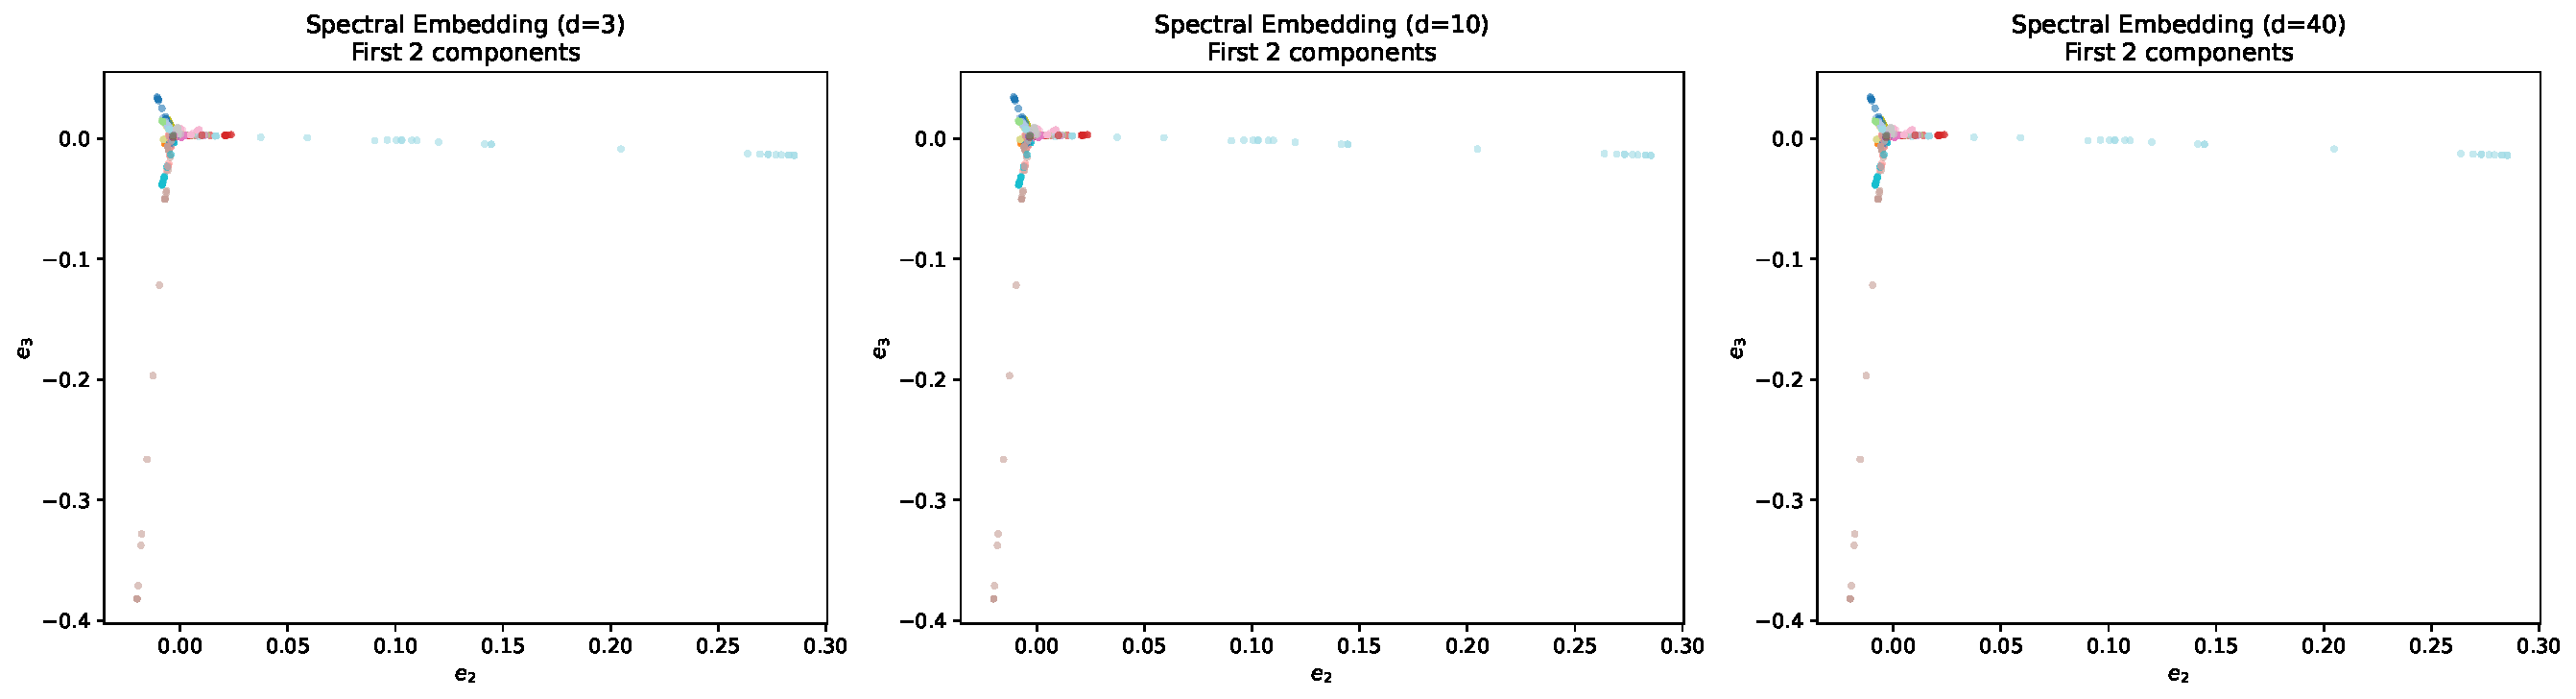
\includegraphics[width=\textwidth]{Figures/ex2d_spectral_embeddings.pdf}
  \caption{Spectral embeddings projected onto the first two coordinates, coloured by Louvain community.}
  \label{fig:ex2d}
\end{figure}

\item We run $k$-means with $k = 29$ (the number of Louvain communities) on each spectral embedding.

\begin{lstlisting}[style=python2]
from sklearn.cluster import KMeans
km = KMeans(n_clusters=29, n_init=20, random_state=42)
labels_d3  = km.fit_predict(X_3)
labels_d10 = km.fit_predict(X_10)
labels_d40 = km.fit_predict(X_40)
\end{lstlisting}

\begin{figure}[H]
  \centering
  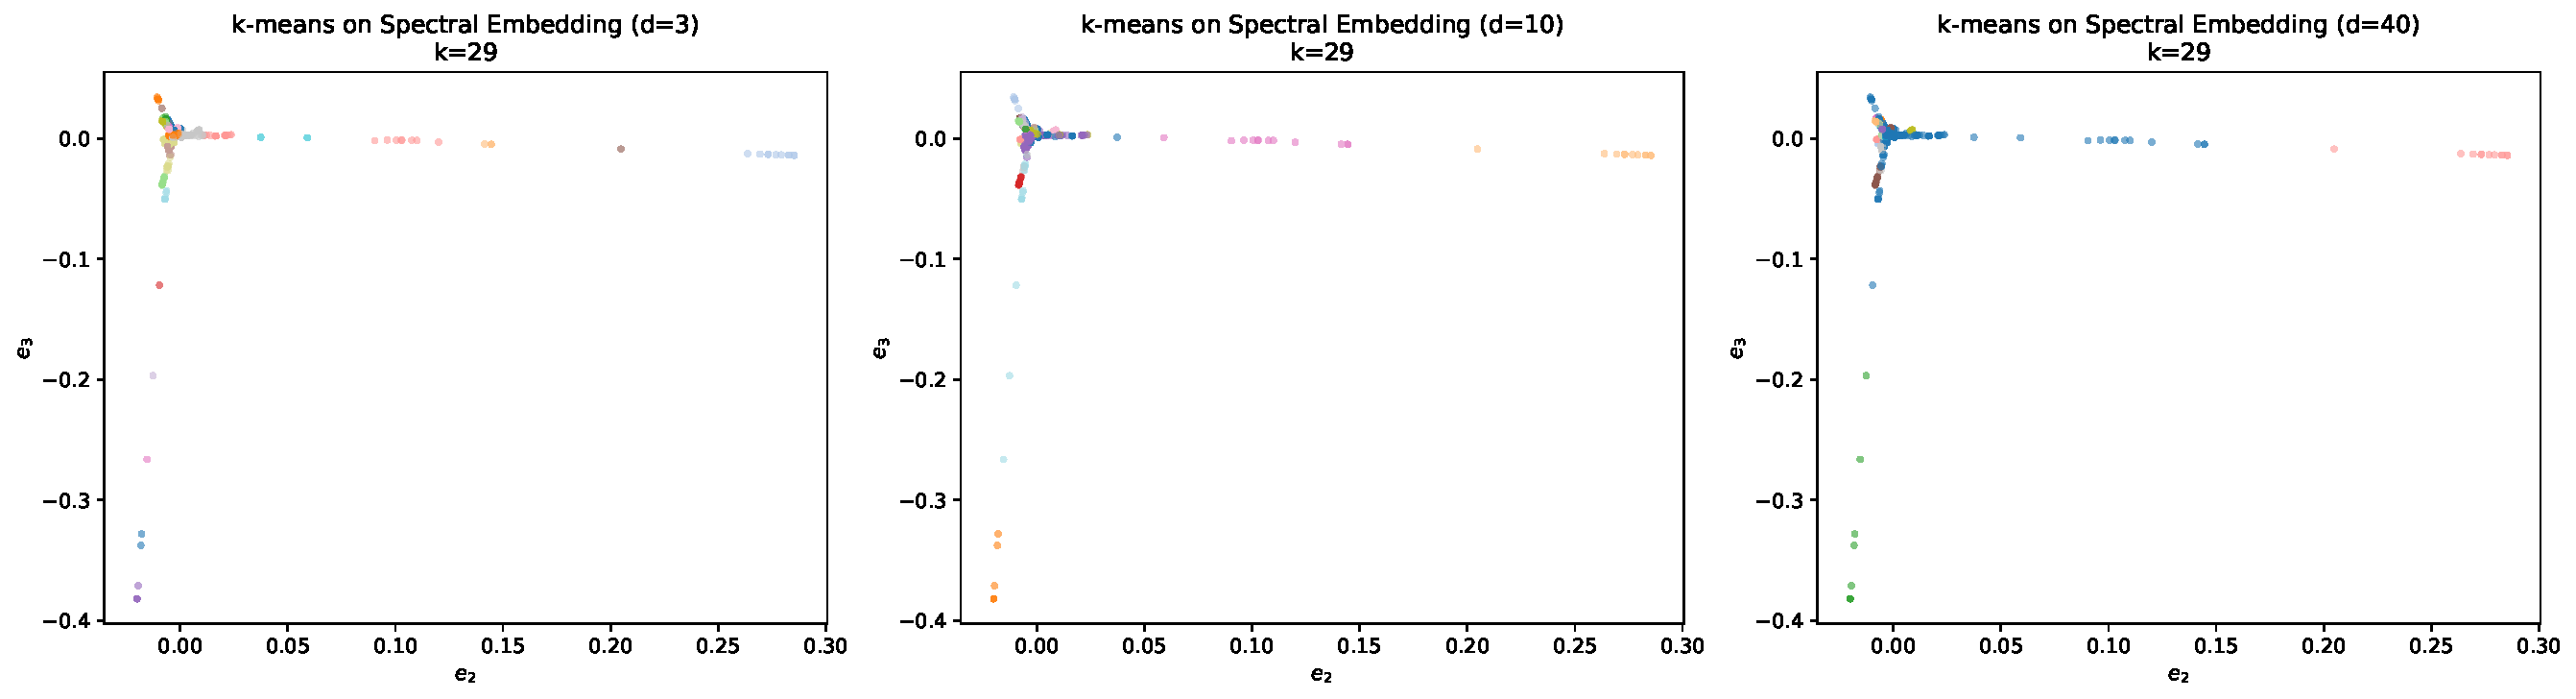
\includegraphics[width=\textwidth]{Figures/ex2e_kmeans_clusters.pdf}
  \caption{$k$-means clusters on spectral embeddings, projected onto the first two coordinates.}
  \label{fig:ex2e}
\end{figure}

\item We compare the Louvain and spectral-$k$-means partitions using \textbf{Normalized Mutual Information (NMI)}, \textbf{Adjusted Rand Index (ARI)}, and \textbf{modularity}.

\begin{center}
\begin{tabular}{l c c c}
\toprule
\textbf{Metric} & $d = 3$ & $d = 10$ & $d = 40$ \\
\midrule
NMI & 0.444 & 0.455 & 0.350 \\
ARI & 0.099 & 0.056 & 0.024 \\
Modularity (spectral) & 0.595 & 0.445 & 0.315 \\
Modularity (Louvain) & \multicolumn{3}{c}{0.817} \\
\bottomrule
\end{tabular}
\end{center}

\begin{figure}[H]
  \centering
  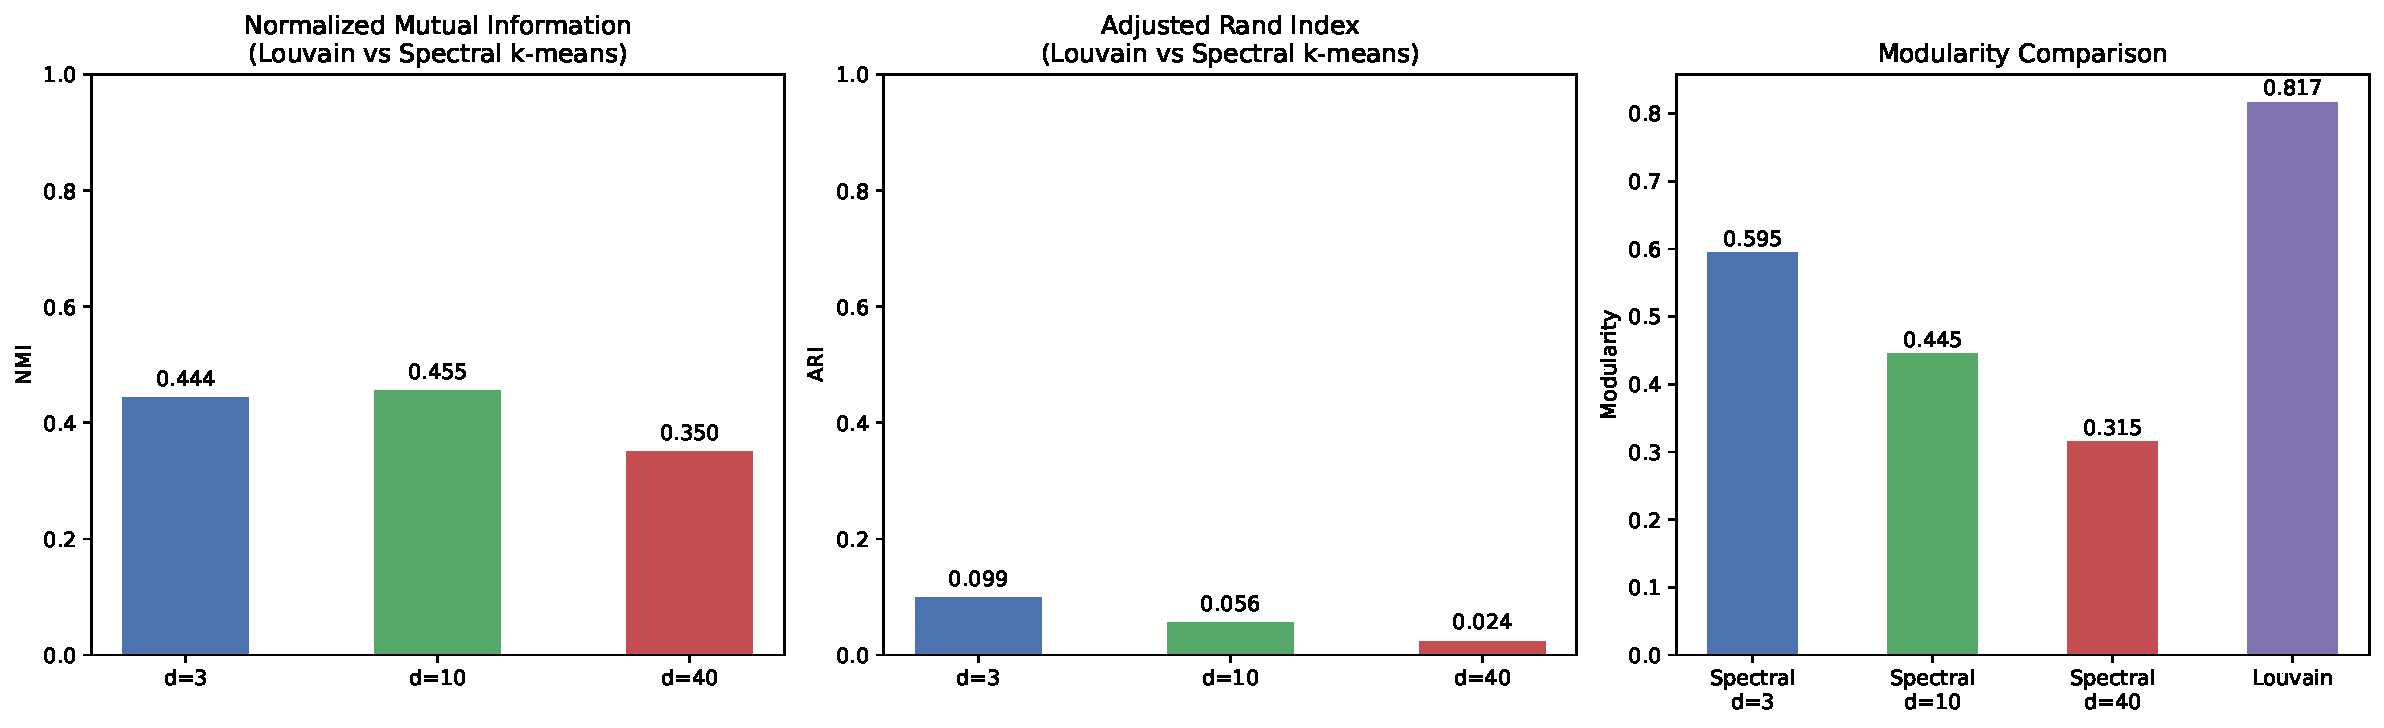
\includegraphics[width=\textwidth]{Figures/ex2f_comparison.pdf}
  \caption{Quantitative comparison of Louvain vs.\ spectral $k$-means clustering.}
  \label{fig:ex2f}
\end{figure}

\textbf{Discussion.}
\begin{itemize}
    \item \textbf{Louvain achieves much higher modularity} ($Q=0.817$) than any spectral-$k$-means partition (best $Q=0.595$ at $d=3$). This is expected: Louvain directly maximizes modularity, whereas spectral clustering optimizes a different objective (graph cuts via the Laplacian spectrum).
    \item \textbf{NMI and ARI are moderate}, indicating partial overlap between the two methods. The best agreement is at $d=10$ (NMI $\approx 0.455$), suggesting the two methods capture some of the same structure but disagree on many vertex assignments.
    \item \textbf{Increasing $d$ does not always help}: $d=10$ gives slightly higher NMI than $d=3$, but $d=40$ performs worst on all metrics. With 29 communities and 1458 vertices, $d=40$ provides too many noisy dimensions for $k$-means (the curse of dimensionality).
    \item \textbf{$d=3$ gives the best spectral modularity} ($0.595$), while $d=40$ drops to $0.315$. The low-dimensional embeddings capture the most informative community structure.
    \item Overall, Louvain is more effective for modularity-based community detection on this network, while spectral methods capture different structural features (e.g., bottleneck/cut-based communities). The two approaches are complementary.
\end{itemize}

\end{enumerate}
\end{tcolorbox}

\vspace{12pt}

\begin{tcolorbox}[colback = gray!16, enhanced, boxrule=0pt, frame hidden, sharp corners, borderline west={3pt}{-1.5pt}{black!80},breakable]
\textbf{Exercise 3 (Cut Metric).} Let $G=(V,E)$ and $G'=(V,E')$ be two graphs on the same vertex set with $|V|=n$. The \textit{cut distance} is defined as:$$d_{\square}(G,G') = \frac{1}{n^2} \min_{\pi \in \mathbb{S}_n} \max_{S,T \subseteq V} \Big| e_G(S,T) - e_{G'}(\pi(S),\pi(T)) \Big|,$$where $\mathbb{S}_n$ is the set of permutations of $\{1, \hdots, n\}$, and $e_G(S,T)$ denotes the number of edges that exist in $G$ between vertex subsets $S$ and $T$.
\begin{enumerate}[$(a)$]
\item Provide an interpretation of the cut metric. What does it capture about the global density of the graphs?

    \item Let $(G_n)$ and $(G'_n)$ be two sequences of graphs such that $d_\square(G_n,G'_n) \to 0$. Prove that the triangle densities converge to the same limit.
    
\textit{(More generally, we actually know that $|t(F,G_n) - t(F,G'_n)| \to 0$ for any motif $F$, where $t(F,G)$ is as defined in lecture.)
}
    \item Let $(G_n)$ and $(G'_n)$ be sequences of graphs sampled from graphons $W$ and $W'$, respectively. Assuming that you can always exchange limits and min/max, determine the limit of $d_\square(G_n,G'_n)$.
    \item Let $(G_n)$ and $(G'_n)$ be two sequences of sparse graphs, such that $|E_n|/n^2 \to 0$ and $|E'_n|/n^2 \to 0$. Prove that $d_\square(G_n,G'_n) \to 0$ always holds. Explain why this implies that the cut metric is uninformative for sparse graphs.
    
\textit{(Thus it turns out the Benjamini-Schramm metric (local convergence) is more appropriate in the sparse regime.)
}    \item We have established that if the motif densities $t(F, G_n)$ converge for all finite graphs $F$, then there exists a graphon $W$ such that $t(F, G_n) \to t(F, W)$. Furthermore, $G_n$ converges to $W$ in the cut metric. Explain why this identifies graphons as the natural limit objects for dense graphs.
\end{enumerate}
\end{tcolorbox}

\begin{tcolorbox}[colback=white, colframe=black!70, title=\textbf{Solution to Exercise 3}, breakable]

\begin{enumerate}[(a)]

\item \textbf{Interpretation of the cut metric.}

The cut distance $d_\square(G,G')$ measures, after optimally relabeling the vertices of one graph via a permutation $\pi \in \S_n$, the maximum discrepancy in the number of edges crossing any bipartite cut $(S,T)$, normalized by $n^2$.

For fixed $\pi$, the quantity $|e_G(S,T) - e_{G'}(\pi(S),\pi(T))|$ measures how differently $G$ and $G'$ distribute edges between two vertex subsets. Maximizing over all $S,T \subseteq V$ finds the bipartite cut that best distinguishes the two graphs, and minimizing over $\pi$ ensures we compare under the best possible vertex alignment.

\boxed{\text{Two graphs are close in } d_\square \text{ iff no bipartite cut can distinguish them after optimal vertex relabeling.}}

This captures \emph{global density structure}: $d_\square(G,G') \approx 0$ means that $G$ and $G'$ have approximately the same edge density between every pair of large vertex subsets, up to relabeling. It is insensitive to local changes (modifying $o(n^2)$ edges does not affect the distance), but detects macroscopic differences in connectivity patterns.

\item \textbf{Convergence of triangle densities.}

Let $t(\triangle, G) = \frac{1}{n^3} \sum_{i,j,k} a_{ij}\, a_{jk}\, a_{ik}$ denote the triangle density. Associate to each graph $G_n$ on $n$ vertices its step-function graphon $W_{G_n}: [0,1]^2 \to \{0,1\}$, defined by partitioning $[0,1]$ into $n$ equal intervals $I_1, \ldots, I_n$ and setting $W_{G_n}(x,y) = a_{ij}$ for $(x,y) \in I_i \times I_j$. Then
\[
t(\triangle, G_n) = t(\triangle, W_{G_n}) = \int_{[0,1]^3} W_{G_n}(x,y)\, W_{G_n}(y,z)\, W_{G_n}(x,z)\, dx\, dy\, dz.
\]
The condition $d_\square(G_n, G_n') \to 0$ implies that there exist permutations $\pi_n$ such that $\|W_{G_n} - W_{G_n'}^{\pi_n}\|_\square \to 0$, where $W_{G_n'}^{\pi_n}$ is the graphon $W_{G_n'}$ with coordinates permuted according to $\pi_n$. Since relabeling does not change triangle density, $t(\triangle, G_n') = t(\triangle, W_{G_n'}^{\pi_n})$.

Write $W = W_{G_n}$ and $U = W_{G_n'}^{\pi_n}$. By multilinearity, expanding $W = U + (W-U)$:
\[
\int W(x,y)W(y,z)W(x,z) - \int U(x,y)U(y,z)U(x,z)
\]
\[
= \int (W{-}U)(x,y)\,W(y,z)\,W(x,z) + \int U(x,y)\,(W{-}U)(y,z)\,W(x,z) + \int U(x,y)\,U(y,z)\,(W{-}U)(x,z).
\]
Each term has the form $\int (W-U)(s,t)\, h(s,t)\, ds\, dt$ after integrating out the third variable, where $\|h\|_\infty \leq 1$. By definition of the cut norm, such integrals are bounded by $\|W - U\|_\square$. Therefore:
\[
\boxed{|t(\triangle, G_n) - t(\triangle, G_n')| \leq 3\,\|W_{G_n} - W_{G_n'}^{\pi_n}\|_\square \leq 3\, d_\square(G_n, G_n') \to 0.}
\]
Hence $t(\triangle, G_n)$ and $t(\triangle, G_n')$ converge to the same limit. $\qed$

\item \textbf{Limit of $d_\square(G_n, G_n')$ for graphs sampled from graphons.}

Let $G_n \sim W$ and $G_n' \sim W'$. As $n \to \infty$, the step-function graphon $W_{G_n}$ converges to $W$ in cut norm (a.s.), and similarly $W_{G_n'} \to W'$. Assuming we may exchange limits and min/max, the discrete minimization over $\pi \in \S_n$ becomes a minimization over measure-preserving bijections $\phi: [0,1] \to [0,1]$, and the discrete max over $S, T$ becomes a sup over measurable $S, T \subseteq [0,1]$:
\[
\boxed{\lim_{n\to\infty} d_\square(G_n, G_n') = \delta_\square(W, W') \,:=\, \inf_{\phi \text{ m.p.}} \|W - W'^\phi\|_\square,}
\]
where $W'^\phi(x,y) = W'(\phi(x), \phi(y))$ and $\|f\|_\square = \sup_{S,T} \l|\int_S \int_T f(x,y)\, dx\, dy\r|$. This is the \textbf{cut distance between graphons}.

\item \textbf{The cut metric is uninformative for sparse graphs.}

For any permutation $\pi$ (in particular $\pi = \mathrm{id}$) and any $S, T \subseteq V$:
\[
|e_{G_n}(S,T) - e_{G_n'}(\pi(S), \pi(T))| \leq e_{G_n}(S,T) + e_{G_n'}(\pi(S), \pi(T)) \leq |E_n| + |E_n'|,
\]
since $e_G(S,T) \leq |E(G)|$ for any $S,T$. Therefore:
\[
\boxed{d_\square(G_n, G_n') \leq \frac{|E_n| + |E_n'|}{n^2} \to 0.}
\]

This means \emph{any} two sparse graph sequences are at cut distance zero, regardless of their structure. A sparse random graph, a sparse expander, a path, and a collection of disjoint triangles all look identical under $d_\square$ as long as $|E|/n^2 \to 0$. The $1/n^2$ normalization is calibrated for dense graphs with $\Theta(n^2)$ edges; sparse graphs with $o(n^2)$ edges are all ``crushed to zero,'' making the cut metric \textbf{uninformative} in the sparse regime. $\qed$

\item \textbf{Graphons as natural limit objects for dense graphs.}

The established equivalence gives two equivalent notions of convergence for dense graph sequences:
\begin{itemize}
    \item \textbf{Motif convergence:} $t(F, G_n)$ converges for every finite graph $F$.
    \item \textbf{Cut metric convergence:} $G_n$ converges to some graphon $W$ in $d_\square$.
\end{itemize}

Their equivalence, combined with the existence of a graphon limit, identifies graphons as the natural limit objects for the following reasons:

\begin{enumerate}[\normalfont 1.]
    \item \textbf{Completeness.} Every convergent sequence of dense graphs (in either sense) has a limit that is a graphon $W \in \mathcal W$, the space of symmetric measurable functions $[0,1]^2 \to [0,1]$. The space of graphons, quotiented by $W \sim W'$ iff $\delta_\square(W,W') = 0$, is a \emph{compact} metric space under $\delta_\square$. Thus graphons form the \textbf{completion} of the space of dense graphs.

    \item \textbf{Universality.} Every graphon can be approximated by a sequence of finite graphs, and every convergent graph sequence has a graphon limit. The set of limit points is exactly the set of graphons (up to measure-preserving equivalence).

    \item \textbf{Analytic tractability.} Graphons encode all asymptotic combinatorial information: for any motif $F$, $t(F, G_n) \to t(F, W) = \int_{[0,1]^{|V(F)|}} \prod_{(i,j)\in E(F)} W(x_i, x_j) \, \prod_i dx_i$. The passage from finite combinatorics to integration on $[0,1]^2$ makes graphons amenable to analysis, probability, and optimization.
\end{enumerate}

\boxed{\text{Graphons are to dense graphs what } \R \text{ is to } \Q\text{: the completion under a natural metric (}d_\square\text{).}}

Just as every Cauchy sequence of rationals converges to a real number, every convergent sequence of dense graphs converges to a graphon, and graphons form the smallest complete space containing all dense graphs.

\end{enumerate}
\end{tcolorbox}


\end{document}